\documentclass[../../main.tex]{subfiles}
\graphicspath{{\subfix{../../image/}}} % 指定图片目录,后续可以直接使用图片文件名。

% 例如:
% \begin{figure}[H]
% \centering
% \includegraphics[scale=0.4]{图.png}
% \caption{}
% \label{figure:图}
% \end{figure}
% 注意:上述\label{}一定要放在\caption{}之后,否则引用图片序号会只会显示??.

\begin{document}

\section{正交多项式}

\subsection{正交函数族与正交多项式}

\begin{definition}
若\( f(x),g(x) \in C[a,b] \),\(\rho(x)\)为\([a,b]\)上的权函数且满足
\begin{align}
(f(x),g(x)) = \int_a^b \rho(x) f(x) g(x) \, \mathrm{d}x = 0, \label{2.1}
\end{align}
则称\( f(x) \)与\( g(x) \)在\([a,b]\)上带权\(\rho(x)\)\textbf{正交}.若函数族\(\varphi_0(x),\varphi_1(x),\cdots,\varphi_n(x),\cdots\)满足关系
\begin{align}
(\varphi_j,\varphi_k) = \int_a^b \rho(x)\varphi_j(x)\varphi_k(x) \, \mathrm{d}x = \begin{cases}
0, & j \neq k, \\
A_k > 0, & j = k.
\end{cases} \label{2.2}
\end{align}
则称\(\{\varphi_k(x)\}\)是\([a,b]\)上带权\(\rho(x)\)的\textbf{正交函数族};若\( A_k \equiv 1 \),则称为\textbf{标准正交函数族}.
\end{definition}

\begin{example}
三角函数族
\[
1,\cos x,\sin x,\cos 2x,\sin 2x,\cdots
\]
就是在区间\([-\pi,\pi]\)上的正交函数族.
\end{example}
\begin{proof}
对\( k=1,2,\cdots \)有
\[
(1,1) = 2\pi, \quad (\sin kx,\sin kx) = (\cos kx,\cos kx) = \pi,
\]
与\( k=1,2,\cdots \)时,
\[
(\cos kx,\sin kx) = (1,\cos kx) = (1,\sin kx) = 0;
\]
而对\( k,j=1,2,\cdots \),当\( k \neq j \)时有
\[
(\cos kx,\cos jx) = (\sin kx,\sin jx) = (\cos kx,\sin jx) = 0.
\]
\end{proof}

\begin{definition}
设$\varphi_n(x)$是$[a,b]$上首项系数$a_n \neq 0$的$n$次多项式,$\rho(x)$为$[a,b]$上的权函数.如果多项式序列$\{\varphi_n(x)\}_{0}^{\infty}$满足关系式
\begin{align*}
(\varphi_j,\varphi_k) = \int_a^b \rho(x)\varphi_j(x)\varphi_k(x) \, \mathrm{d}x = \begin{cases}
0, & j \neq k, \\
A_k > 0, & j = k.
\end{cases}
\end{align*}
则称多项式序列$\{\varphi_n(x)\}_{0}^{\infty}$为在$[a,b]$上带权$\rho(x)$\textbf{正交},称$\varphi_n(x)$为$[a,b]$上\textbf{带权$\boldsymbol{\rho }\mathbf{(}\boldsymbol{x}\mathbf{)}$的$\boldsymbol{n}$次正交多项式}.
\end{definition}

\begin{theorem}
若给定区间$[a,b]$及权函数$\rho(x)$,则可由一族线性无关的幂函数$\{1,x,\cdots,x^n,\cdots\}$,利用逐个正交化手续构造出正交多项式序列$\{\varphi_n(x)\}_{0}^{\infty}$:
\begin{align}
\varphi_0(x) &= 1, \nonumber \\
\varphi_n(x) &= x^n - \sum_{j=0}^{n-1} \frac{(x^n, \varphi_j(x))}{(\varphi_j(x), \varphi_j(x))} \varphi_j(x),\quad n=1,2,\cdots.\label{eq:数值分析-3-2.3}
\end{align}
这样得到的正交多项式$\varphi_n(x)$,其最高项系数为$1$.

反之,若$\{\varphi_n(n)\}_{0}^{\infty}$是正交多项式,则$\varphi_0(x),\varphi_1(x),\cdots,\varphi_n(x)$在$[a,b]$上是线性无关的.
\end{theorem}
\begin{proof}
容易验证逐个正交化得到的多项式序列$\{\varphi_n(x)\}_{0}^{\infty}$在$[a,b]$上带权$\rho(x)$正交,且其最高项系数为1.

反之,若
$$c_0\varphi_0(x) + c_1\varphi_1(x) + \cdots + c_n\varphi_n(x) = 0,$$
用$\rho(x)\varphi_j(x)$($j=0,1,\cdots,n$)乘上式并积分得
\begin{align*}
&c_0\int_a^b{\rho (x)\varphi _0(x)\varphi _j(x)\mathrm{d}x}+c_1\int_a^b{\rho (x)\varphi _1(x)\varphi _j(x)\mathrm{d}x}+\cdots 
\\
&+c_j\int_a^b{\rho (x)\varphi _j(x)\varphi _j(x)\mathrm{d}x}+\cdots +c_n\int_a^b{\rho (x)\varphi _n(x)\varphi _j(x)\mathrm{d}x}=0.
\end{align*}
利用正交性有
$$c_j\int_a^b \rho(x)\varphi_j(x)\varphi_j(x)\mathrm{d}x = 0.$$
由于$(\varphi_j,\varphi_j) = \int_a^b \rho(x)\varphi_j^2(x)\mathrm{d}x > 0$,故$c_j = 0$对$j=0,1,\cdots,n$成立.由此得出$\varphi_0(x),\varphi_1(x),\cdots,\varphi_n(x)$线性无关.
\end{proof}

\begin{theorem}\label{theorem:正交多项式的性质}
设$\{\varphi_n(x)\}_{0}^{\infty}$是$[a,b]$上带权$\rho(x)$的正交多项式,则
\begin{enumerate}
\item 对任何$P(x) \in H_n$均可表示为$\varphi_0(x),\varphi_1(x),\cdots,\varphi_n(x)$的线性组合,即
$$P(x) = \sum_{j=0}^n c_j\varphi_j(x).$$
其中$c_0,c_1,\cdots,c_n$不全为0.

\item $\varphi_n(x)$与任何次数小于$n$的多项式$P(x) \in H_{n-1}$正交,即
$$(\varphi_n, P) = \int_a^b \rho(x)\varphi_n(x)P(x)\mathrm{d}x = 0.$$
\end{enumerate}
\end{theorem}
\begin{proof}

\end{proof}

\begin{theorem}
设$\{\varphi_n(x)\}_{0}^{\infty}$是$[a,b]$上带权$\rho(x)$的正交多项式,对$n \geq 0$成立递推关系
\begin{align}\label{eq:数值分析-3-2.4}
\varphi_{n+1}(x) = (x - \alpha_n)\varphi_n(x) - \beta_n\varphi_{n-1}(x),\quad n = 0,1,\cdots,
\end{align}
其中
\begin{align*}
&\varphi _0(x)=1,\quad \varphi _{-1}(x)=0,
\\
&\alpha _n=(x\varphi _n(x),\varphi _n(x))/(\varphi _n(x),\varphi _n(x)),
\\
&\beta _n=(\varphi _n(x),\varphi _n(x))/(\varphi _{n-1}(x),\varphi _{n-1}(x)),\quad n=1,2,\cdots ,
\end{align*}
这里$(x\varphi_n(x),\varphi_n(x)) = \int_a^b x\varphi_n^2(x)\rho(x)\mathrm{d}x$.
\end{theorem}
\begin{proof}

\end{proof}

\begin{theorem}
设$\{\varphi_n(x)\}_{0}^{\infty}$是$[a,b]$上带权$\rho(x)$的正交多项式,则$\varphi_n(x)$($n \geq 1$)在区间$(a,b)$内有$n$个不同的零点.
\end{theorem}
\begin{proof}
假定$\varphi_n(x)$在$(a,b)$内的零点都是偶数重的,则$\varphi_n(x)$在$[a,b]$上符号保持不变.这与
$$(\varphi_n,\varphi_0) = \int_a^b \rho(x)\varphi_n(x)\varphi_0(x)\mathrm{d}x = 0$$
矛盾.故$\varphi_n(x)$在$(a,b)$内的零点不可能全是偶重的,现设$x_i$($i=1,2,\cdots,l$)为$\varphi_n(x)$在$(a,b)$内的奇数重零点,不妨设
$$a < x_1 < x_2 < \cdots < x_l < b,$$
则$\varphi_n(x)$在$x_i$($i=1,2,\cdots,l$)处变号.令
$$q(x) = (x - x_1)(x - x_2)\cdots(x - x_l),$$
于是$\varphi_n(x)q(x)$在$[a,b]$上不变号,则得
$$(\varphi_n,q) = \int_a^b \rho(x)\varphi_n(x)q(x)\mathrm{d}x \neq 0.$$
若$l < n$,由$\{\varphi_n(x)\}_{0}^{\infty}$的正交性可知
$$(\varphi_n,q) = \int_a^b \rho(x)\varphi_n(x)q(x)\mathrm{d}x = 0,$$
与$(\varphi_n,q) \neq 0$矛盾,故$l \geq n$.而$\varphi_n(x)$只有$n$个零点,故$l = n$,即$n$个零点都是单重的.证毕.
\end{proof}


\subsection{Legendre(勒让德)多项式}

\begin{definition}[Legendre(勒让德)多项式]
当区间为$[-1,1]$,权函数$\rho(x) \equiv 1$时,由$\{1,x,\cdots,x^n,\cdots\}$正交化得到的多项式称为\textbf{勒让德(Legendre)多项式},并用$P_0(x),P_1(x),\cdots,P_n(x),\cdots$表示.这是勒让德于1785年引进的.1814年\textbf{罗德利克(Rodrigul)}给出了勒让德多项式的简单表达式
\begin{align}\label{eq:数值分析-3-2.5}
P_0(x) = 1,\quad P_n(x) = \frac{1}{2^n n!} \frac{\mathrm{d}^n}{\mathrm{d}x^n}(x^2 - 1)^n,\quad n = 1,2,\cdots.
\end{align}
由于$(x^2 - 1)^n$是$2n$次多项式,求$n$阶导数后得
$$P_n(x) = \frac{1}{2^n n!}(2n)(2n - 1)\cdots(n + 1)x^n + a_{n-1}x^{n-1} + \cdots + a_0,$$
于是得首项$x^n$的系数$a_n = \frac{(2n)!}{2^n (n!)^2}$.显然最高项系数为1的勒让德多项式为
\begin{align}\label{eq:数值分析-3-2.6}
\widetilde{P}_0(x) = 1,\quad \widetilde{P}_n(x) &= \frac{n!}{(2n)!} \frac{\mathrm{d}^n}{\mathrm{d}x^n}(x^2 - 1)^n,\quad n = 1,2,\cdots.
\end{align}
\end{definition}

\begin{theorem}[Legendre多项式的性质]\label{theorem:Legendre多项式的性质}
设$\{P_n(x)\}_0^{\infty}$是Legendre多项式,它可表示为
\begin{align*}
P_0(x) = 1,\quad P_n(x) = \frac{1}{2^n n!} \frac{\mathrm{d}^n}{\mathrm{d}x^n}(x^2 - 1)^n,\quad n = 1,2,\cdots.
\end{align*}
则有
\begin{enumerate}
\item (正交性)
\begin{align}\label{eq:数值分析-3-2.7}
\int_{-1}^1 P_n(x)P_m(x)\mathrm{d}x &=
\begin{cases}
0, & m \neq n; \\
\dfrac{2}{2n+1}, & m = n.
\end{cases}
\end{align}

\item (奇偶性)
\begin{align}\label{eq:数值分析-3-2.8}
P_n(-x) &= (-1)^n P_n(x).
\end{align}

\item (递推关系)
\begin{align}\label{eq:数值分析-3-2.9}
(n+1)P_{n+1}(x) &= (2n+1)xP_n(x) - nP_{n-1}(x),\quad n = 1,2,\cdots.
\end{align}

\item $P_n(x)$在区间$[-1,1]$内有$n$个不同的实零点.
\end{enumerate}
\end{theorem}
\begin{proof}
\begin{enumerate}
\item 令$\varphi(x) = (x^2 - 1)^n$,则
$$\varphi^{(k)}(\pm 1) = 0,\quad k = 0,1,\cdots,n-1.$$
设$Q(x)$是在区间$[-1,1]$上有$n$阶连续可微的函数,由分部积分法知
\begin{align*}
\int_{-1}^1 P_n(x)Q(x)\mathrm{d}x &= \frac{1}{2^n n!}\int_{-1}^1 Q(x)\varphi^{(n)}(x)\mathrm{d}x = -\frac{1}{2^n n!}\int_{-1}^1 Q'(x)\varphi^{(n-1)}(x)\mathrm{d}x \\
&= \cdots = \frac{(-1)^n}{2^n n!}\int_{-1}^1 Q^{(n)}(x)\varphi(x)\mathrm{d}x.
\end{align*}
下面分两种情况讨论.

(1)若$Q(x)$是次数小于$n$的多项式,则$Q^{(n)}(x) \equiv 0$,故得
$$\int_{-1}^1 P_n(x)P_m(x)\mathrm{d}x = 0,\quad \text{当 } n \neq m.$$

(2)若
$$Q(x) = P_n(x) = \frac{1}{2^n n!}\varphi^{(n)}(x) = \frac{(2n)!}{2^n (n!)^2}x^n + \cdots,$$
则
$$Q^{(n)}(x) = P_n^{(n)}(x) = \frac{(2n)!}{2^n n!},$$
于是
$$\int_{-1}^1 P_n^2(x)\mathrm{d}x = \frac{(-1)^n (2n)!}{2^{2n} (n!)^2}\int_{-1}^1 (x^2 - 1)^n \mathrm{d}x = \frac{(2n)!}{2^{2n} (n!)^2}\int_{-1}^1 (1 - x^2)^n \mathrm{d}x.$$
由于
$$\int_{0}^1 (1 - x^2)^n \mathrm{d}x = \int_{0}^{\frac{\pi}{2}} \cos^{2n+1}t \mathrm{d}t = \frac{2 \cdot 4 \cdot \cdots \cdot (2n)}{1 \cdot 3 \cdot \cdots \cdot (2n+1)},$$
故
$$\int_{-1}^1 P_n^2(x)\mathrm{d}x = \frac{2}{2n+1},$$
于是\eqref{eq:数值分析-3-2.7}式得证.

\item 由于$\varphi(x) = (x^2 - 1)^n$是偶次多项式,经过偶次求导仍为偶次多项式,经过奇次求导仍为奇次多项式,故$n$为偶数时$P_n(x)$为偶函数,$n$为奇数时$P_n(x)$为奇函数,于是\eqref{eq:数值分析-3-2.8}式成立.

\item 考虑$n+1$次多项式$xP_n(x)$,它可表示为
$$xP_n(x) = a_0P_0(x) + a_1P_1(x) + \cdots + a_{n+1}P_{n+1}(x).$$
两边乘$P_k(x)$,并从$-1$到$1$积分,并利用正交性得
$$\int_{-1}^1 xP_n(x)P_k(x)\mathrm{d}x = a_k\int_{-1}^1 P_k^2(x)\mathrm{d}x.$$
当$k \leq n-2$时,$xP_k(x)$次数小于等于$n-1$,上式左端积分为$0$,故得$a_0 = 0$.当$k = n$时,$xP_n^2(x)$为奇函数,左端积分仍为$0$,故$a_n = 0$.于是
$$xP_n(x) = a_{n-1}P_{n-1}(x) + a_{n+1}P_{n+1}(x),$$
其中
\begin{align*}
a_{n-1} &= \frac{2n-1}{2}\int_{-1}^1 xP_n(x)P_{n-1}(x)\mathrm{d}x \\
&= \frac{2n-1}{2} \cdot \frac{2n}{4n^2 - 1} = \frac{n}{2n+1},
\end{align*}
\begin{align*}
a_{n+1} &= \frac{2n+3}{2}\int_{-1}^1 xP_n(x)P_{n+1}(x)\mathrm{d}x \\
&= \frac{2n+3}{2} \cdot \frac{2(n+1)}{(2n+1)(2n+3)} = \frac{n+1}{2n+1},
\end{align*}
从而得到以下的递推公式
\begin{align}\label{eq:数值分析-3-2..9}
(n+1)P_{n+1}(x) &= (2n+1)xP_n(x) - nP_{n-1}(x),\quad n = 1,2,\cdots.
\end{align}
由$P_0(x) = 1$,$P_1(x) = x$,利用\eqref{eq:数值分析-3-2..9}式就可推出
\begin{align*}
&P_2(x)=(3x^2-1)/2,
\\
&P_3(x)=(5x^3-3x)/2,
\\
&P_4(x)=(35x^4-30x^2+3)/8,
\\
&P_5(x)=(63x^5-70x^3+15x)/8,
\\
&P_6(x)=(231x^6-315x^4+105x^2-5)/16,
\\
&\vdots 
\end{align*}
\reffig{figure:Legendre多项式图1}给出了$P_0(x)$,$P_1(x)$,$P_2(x)$,$P_3(x)$的图形.\begin{figure}[H]
\centering
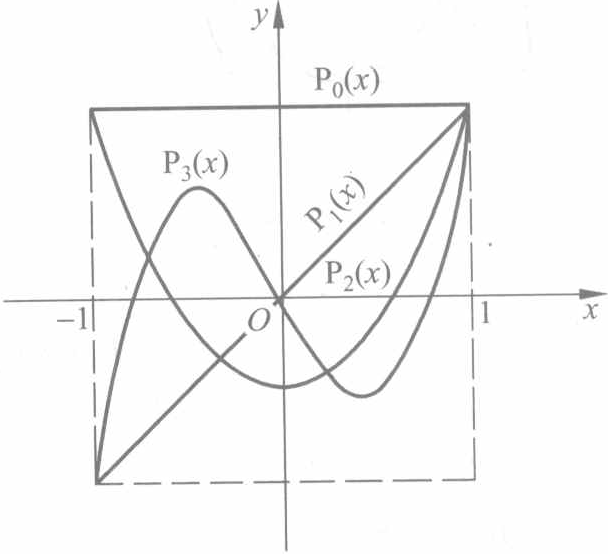
\includegraphics[scale=0.4]{Legendre多项式图1.png}
\caption{}
\label{figure:Legendre多项式图1}
\end{figure}

\item 
\end{enumerate}
\end{proof}


\subsection{Chebeshev(切比雪夫)多项式}

\begin{definition}[Chebeshev(切比雪夫)多项式]
当权函数$\rho(x) = \dfrac{1}{\sqrt{1 - x^2}}$,区间为$[-1,1]$时,由序列$\{1,x,\cdots,x^n,\cdots\}$正交化得到的正交多项式就是\textbf{Chebeshev(切比雪夫)多项式},它可表示为
\begin{align}\label{eq:数值分析-3-2.10}
T_n(x) &= \cos(n \arccos x),\quad |x| \leq 1.
\end{align}
若令$x = \cos\theta$,则$T_n(x) = \cos n\theta$,$0 \leq \theta \leq \pi$.
\end{definition}
\begin{remark}
由于切比雪夫多项式是在区间$[-1,1]$上定义的,对于一般区间$[a,b]$,要通过变量替换变换到$[-1,1]$,可令
\begin{align}\label{eq:数值分析-3-2.14}
x &= \frac{1}{2}[(b - a)t + a + b],
\end{align}
则可将$x \in [a,b]$变换到$t \in [-1,1]$.
\end{remark}

\begin{theorem}[Chebeshev多项式的性质]\label{theorem:Chebeshev多项式的性质}
设$\{T_n(x)\}$是Chebeshev多项式,它可表示为
\begin{align*}
T_n(x) &= \cos(n \arccos x),\quad |x| \leq 1,\quad n=1,2,\cdots.
\end{align*}
则有
\begin{enumerate}
\item (递推关系)
\begin{align}\label{eq:数值分析-3-2.11}
&\begin{cases}
T_{n+1}(x) = 2xT_n(x) - T_{n-1}(x),\quad n = 1,2,\cdots, \\
T_0(x) = 1,\quad T_1(x) = x.
\end{cases}
\end{align}

\item $T_n(x)$的首项$x^n$的系数为$2^{n-1}$($n=1,2,\cdots$),进而若令
\begin{align*}
\widetilde{T}_0(x) = 1,\widetilde{T}_n(x) = \frac{1}{2^{n-1}}T_n(x),n=1,2,\cdots,
\end{align*}
则$\widetilde{T}_n(x)$是首项系数为1的Chebeshev多项式.

\item $T_{2k}(x)$只含$x$的偶次幂,$T_{2k+1}(x)$只含$x$的奇次幂.

\item Chebeshev多项式$\{T_k(x)\}$在区间$[-1,1]$上带权$\rho(x) = \frac{1}{\sqrt{1 - x^2}}$正交,且
\begin{align}\label{eq:数值分析-3-2.12}
\int_{-1}^1 \frac{T_n(x)T_m(x)}{\sqrt{1 - x^2}}\mathrm{d}x &=
\begin{cases}
0, & n \neq m; \\
\dfrac{\pi}{2}, & n = m \neq 0; \\
\pi, & n = m = 0.
\end{cases}
\end{align}

\item $T_n(x)$在区间$[-1,1]$上有$n$个零点
$$x_k = \cos\frac{2k - 1}{2n}\pi,\quad k = 1,2,\cdots,n.$$
和$n+1$个极值点(包括端点)
$$x_k = \cos\frac{k\pi}{n},\quad k = 0,1,\cdots,n.$$
这两组点称为\textbf{Chebeshev(切比雪夫)点}.
\end{enumerate}
\end{theorem}
\begin{proof}
\begin{enumerate}
\item 这只要由三角恒等式
$$\cos(n+1)\theta = 2\cos\theta\cos n\theta - \cos(n-1)\theta,\quad n = 1,2,\cdots,$$
令$x = \cos\theta$即得.由\eqref{eq:数值分析-3-2.11}式就可推出
\begin{align*}
&T_2(x)=2x^2-1,
\\
&T_3(x)=4x^3-3x,
\\
&T_4(x)=8x^4-8x^2+1,
\\
&T_5(x)=16x^5-20x^3+5x,
\\
&T_6(x)=32x^6-48x^4+18x^2-1,
\\
&\vdots 
\end{align*}

函数$T_0(x)$,$T_1(x)$,$T_2(x)$,$T_3(x)$的图形见\reffig{figure:Chebeshev多项式图1}.
\begin{figure}[H]
\centering
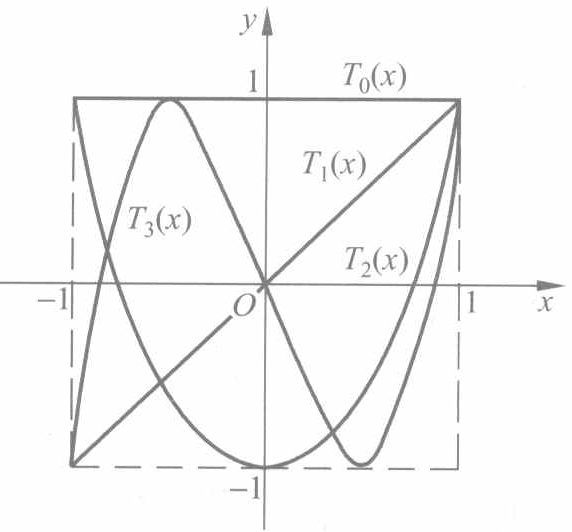
\includegraphics[scale=0.4]{Chebeshev多项式图1.png}
\caption{}
\label{figure:Chebeshev多项式图1}
\end{figure}

\item 此性质可由递推关系\eqref{eq:数值分析-3-2.11}归纳得到.

\item 此性质也可由递推关系\eqref{eq:数值分析-3-2.11}归纳得到.

\item 事实上,令$x = \cos\theta$,则$\mathrm{d}x = -\sin\theta\mathrm{d}\theta$,于是
$$\int_{-1}^1 \frac{T_n(x)T_m(x)}{\sqrt{1 - x^2}}\mathrm{d}x = \int_0^\pi \cos n\theta\cos m\theta\mathrm{d}\theta =
\begin{cases}
0, & n \neq m; \\
\dfrac{\pi}{2}, & n = m \neq 0; \\
\pi, & n = m = 0.
\end{cases}$$

\item 
\end{enumerate}
\end{proof}

\begin{theorem}\label{theorem:数值分析-3-定理6}
设$\widetilde{T}_n(x)$是首项系数为1的切比雪夫多项式,记$\widetilde{H}_n$为所有次数小于等于$n$的首项系数为1的多项式集合,则
$$\max_{-1 \leqslant x \leqslant 1} |\widetilde{T}_n(x)| \leqslant \max_{-1 \leqslant x \leqslant 1} |P(x)|,\quad \forall P(x) \in \widetilde{H}_n,$$
且
$$\max_{-1 \leqslant x \leqslant 1} |\widetilde{T}_n(x)| = \frac{1}{2^{n-1}}.$$
\end{theorem}
\begin{note}
这个定理表明在所有首项系数为1的$n$次多项式集合$\widetilde{H}_n$中
$$\|\widetilde{T}_n\|_\infty = \min_{P \in \widetilde{H}_n} \|P(x)\|_\infty,$$
所以$\widetilde{T}_n(x)$是$\widetilde{H}_n$中最大值最小的多项式,即
\begin{align}\label{eq:数值分析-3-2.13}
\max_{-1 \leq x \leq 1} |\widetilde{T}_n(x)| = \min_{P \in \widetilde{H}_n} \max_{-1 \leq x \leq 1} |P(x)| = \frac{1}{2^{n-1}}.
\end{align}
利用这一结论,可求$P(x) \in H_n$在$H_{n-1}$中的最佳(一致)逼近多项式.
\end{note}
\begin{proof}

\end{proof}

\begin{example}
求$f(x) = 2x^3 + x^2 + 2x - 1$在$[-1,1]$上的最佳二次逼近多项式.
\end{example}
\begin{solution}
由题意,所求最佳逼近多项式$P_2^*(x)$应满足
$$\max_{-1 \leq x \leq 1} |f(x) - P_2^*(x)| = \min.$$
由\refthe{theorem:数值分析-3-定理6}可知,当
$$f(x) - P_2^*(x) = \frac{1}{2}T_3(x) = 2x^3 - \frac{3}{2}x$$
时,多项式$f(x) - P_2^*(x)$与零偏差最小,故
$$P_2^*(x) = f(x) - \frac{1}{2}T_3(x) = x^2 + \frac{7}{2}x - 1$$
就是$f(x)$在$[-1,1]$上的最佳二次逼近多项式.
\end{solution}


\subsection{Chebeshev多项式零点插值}

\hyperref[theorem:Chebeshev多项式的性质]{Chebeshev(切比雪夫)点}在插值中有重要作用.从\reffig{figure:Chebeshev点}可以看到切比雪夫点恰好是单位圆周上等距分布点的横坐标,这些点的横坐标在接近区间$[-1,1]$的端点处是密集的.
\begin{figure}[H]
\centering
\includegraphics[scale=0.4]{Chebeshev点.png}
\caption{}
\label{figure:Chebeshev点}
\end{figure}

\begin{theorem}
设插值节点$x_0,x_1,\cdots,x_n$为切比雪夫多项式$T_{n+1}(x)$的零点,被插函数$f \in C^{n+1}[-1,1]$,$L_n(x)$为相应的插值多项式,则
\begin{align}\label{eq:数值分析-3-2.15}
\max_{-1 \leq x \leq 1} |f(x) - L_n(x)| &\leq \frac{1}{2^n (n+1)!}\|f^{(n+1)}(x)\|_\infty.
\end{align}
对于一般区间$[a,b]$上的插值只要利用变换\eqref{eq:数值分析-3-2.14}式则可得到相应结果
\begin{align*}
\max_{a \leq x \leq b} |f(x) - L_n(x)| &\leq \frac{1}{2^n (n+1)!}\|f^{(n+1)}(x)\|_\infty.
\end{align*}
此时插值节点为
$$x_k = \frac{b - a}{2}\cos\frac{2k+1}{2(n+1)}\pi + \frac{a + b}{2},\quad k = 0,1,\cdots,n.$$
\end{theorem}
\begin{note}
对\eqref{eq:数值分析-3-2.15}式令$n\to \infty$则误差趋于0. 因此这个定理表明:利用切比雪夫点做插值,可使插值区间最大误差最小化.
\end{note}
\begin{proof}
由\refthe{theorem:Lagrange插值多项式的Lagrange插值余项}知插值余项
$$R_n(x) = f(x) - L_n(x) = \frac{f^{(n+1)}(\xi)}{(n+1)!}\omega_{n+1}(x),$$
这里 $\xi \in (a, b)$ 且依赖于 $x$,$\,\,\omega_{n + 1}(x)$ 由 \eqref{eq:数值分析-2.10} 式所定义。于是
$$\max_{-1 \leq x \leq 1} |f(x) - L_n(x)| \leq \frac{M_{n+1}}{(n+1)!}\max_{-1 \leq x \leq 1} |(x - x_0)(x - x_1)\cdots(x - x_n)|,$$
其中
$$M_{n+1} = \|f^{(n+1)}(x)\|_\infty = \max_{-1 \leq x \leq 1} |f^{(n+1)}(x)|$$
是由被插函数确定的.因为插值节点为$T_{n+1}(x)$的零点
$$x_k = \cos\frac{2k+1}{2(n+1)}\pi,\quad k = 0,1,\cdots,n,$$
所以$\omega_{n+1}(x)$就是首先系数为1的Chebeshev多项式.由\eqref{eq:数值分析-3-2.13}式可得
$$\max_{-1 \leq x \leq 1} |\omega_{n+1}(x)| = \max_{-1 \leq x \leq 1} |\widetilde{T}_{n+1}(x)| = \frac{1}{2^n}.$$
由此可得\eqref{eq:数值分析-3-2.15}.
\end{proof}

\begin{example}
求$f(x) = \mathrm{e}^x$在$[0,1]$上的四次拉格朗日插值多项式$L_4(x)$,插值节点用$T_5(x)$的零点,并估计误差$\max\limits_{0 \leq x \leq 1} |\mathrm{e}^x - L_4(x)|$.
\end{example}
\begin{solution}
利用$T_5(x)$的零点和区间变换可知节点
$$x_k = \frac{1}{2}\left(1 + \cos\frac{2k+1}{10}\pi\right),\quad k = 0,1,2,3,4,$$
即
$$x_0 = 0.97553,\quad x_1 = 0.79390,\quad x_2 = 0.5,$$
$$x_3 = 0.20611,\quad x_4 = 0.02447.$$
对应的拉格朗日插值多项式为
$$L_4(x) = 1.00002274 + 0.99886233x + 0.50902251x^2 + 0.14184105x^3 + 0.06849435x^4.$$
利用\eqref{eq:数值分析-3-2.15}式可得误差估计
$$\max\limits_{0 \leq x \leq 1} |\mathrm{e}^x - L_4(x)| \leq \frac{M_{n+1}}{(n+1)!} \frac{(b - a)^{n+1}}{2^{2n+1}},\quad n = 4,$$
而
$$M_{n+1} = \|f^{(5)}(x)\|_\infty \leq \|\mathrm{e}^x\|_\infty \leq \mathrm{e}^1 \leq 2.72,$$
于是有
$$\max\limits_{0 \leq x \leq 1} |\mathrm{e}^x - L_4(x)| \leq \frac{\mathrm{e}}{5!} \frac{1}{2^9} < \frac{2.72}{6} \frac{1}{10240} < 4.4 \times 10^{-5}.$$
\end{solution}

在\hyperref[高次插值导致的龙格现象]{第2章}中已经知道,由于高次插值出现龙格现象,一般$L_n(x)$不收敛于$f(x)$,因此它并不适用.但若用切比雪夫多项式零点插值却可避免龙格现象,可保证整个区间上收敛.

\begin{example}
设$f(x) = \frac{1}{1 + x^2}$,在$[-5,5]$上利用$T_{11}(x)$的零点作插值点,构造10次拉格朗日插值多项式$\widetilde{L}_{10}(x)$.与第2章得到的等距节点造出的$L_{10}(x)$近似$f(x)$作比较.
\end{example}
\begin{solution}
在$[-1,1]$上的11次切比雪夫多项式$T_{11}(x)$的零点为
$$t_k = \cos\frac{21 - 2k}{22}\pi,\quad k = 0,1,\cdots,10.$$
作变换$x_k = 5t_k$,$k = 0,1,\cdots,10$.它们是$(-5,5)$内的插值点,由此得到$y = f(x)$在$[-5,5]$上的拉格朗日插值多项式$\widetilde{L}_{10}(x)$,$f(x)$,$L_{10}(x)$,$\widetilde{L}_{10}(x)$的图形见\reffig{figure:Chebeshev零点插值示例图},从图中看到$\widetilde{L}_{10}(x)$没有出现龙格现象.
\begin{figure}[H]
\centering
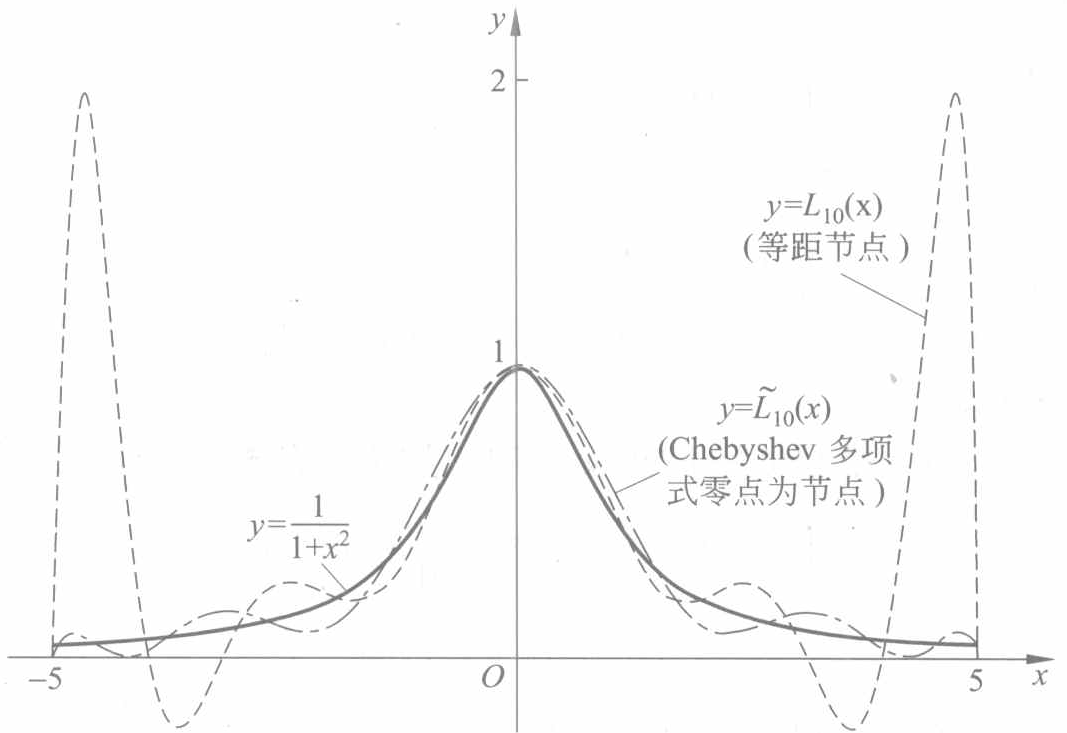
\includegraphics[scale=0.3]{Chebeshev零点插值示例图.png}
\caption{}
\label{figure:Chebeshev零点插值示例图}
\end{figure}
\end{solution}


\subsection{其他常用的正交多项式}

\begin{definition}[第二类切比雪夫多项式]\label{definition:第二类切比雪夫多项式}
在区间$[-1,1]$上带权$\rho(x) = \sqrt{1 - x^2}$的正交多项式称为\textbf{第二类切比雪夫多项式},其表达式为
\begin{align}\label{eq:数值分析-3-2.16}
U_n(x) &= \frac{\sin[(n + 1)\arccos x]}{\sqrt{1 - x^2}}.
\end{align}
\end{definition}

\begin{theorem}
$\{U_n(x)\}$是$[-1,1]$上带权$\sqrt{1 - x^2}$的正交多项式族.并且还有递推关系式
$$U_0(x) = 1,\quad U_1(x) = 2x,$$
$$U_{n+1}(x) = 2xU_n(x) - U_{n-1}(x),\quad n = 1,2,\cdots.$$
\end{theorem}
\begin{proof}
令$x = \cos\theta$,可得
$$\int_{-1}^1 U_n(x)U_m(x)\sqrt{1 - x^2}\mathrm{d}x = \int_0^\pi \sin(n + 1)\theta\sin(m + 1)\theta\mathrm{d}\theta =
\begin{cases}
0, & m \neq n, \\
\dfrac{\pi}{2}, & m = n,
\end{cases}$$
故$\{U_n(x)\}$是$[-1,1]$上带权$\sqrt{1 - x^2}$的正交多项式族.
\end{proof}

\begin{definition}[Laguerre(拉盖尔)多项式]
在区间$[0,+\infty)$上带权$\mathrm{e}^{-x}$的正交多项式称为\textbf{Laguerre(拉盖尔)多项式},其表达式为
\begin{align}\label{eq:数值分析-3-2.17}
\mathrm{L}_n(x) &= \mathrm{e}^x \frac{\mathrm{d}^n}{\mathrm{d}x^n}(x^n \mathrm{e}^{-x}).
\end{align}
\end{definition}

\begin{theorem}
Laguerre(拉盖尔)多项式也具有正交性质
$$\int_0^\infty \mathrm{e}^{-x}\mathrm{L}_n(x)\mathrm{L}_m(x)\mathrm{d}x =
\begin{cases}
0, & m \neq n, \\
(n!)^2, & m = n,
\end{cases}$$
和递推关系
$$\mathrm{L}_0(x) = 1,\quad \mathrm{L}_1(x) = 1 - x,$$
$$\mathrm{L}_{n+1}(x) = (1 + 2n - x)\mathrm{L}_n(x) - n^2\mathrm{L}_{n-1}(x),\quad n = 1,2,\cdots.$$
\end{theorem}
\begin{proof}

\end{proof}

\begin{definition}[Hermite(埃尔米特)多项式]
在区间$(-\infty,+\infty)$上带权$\mathrm{e}^{-x^2}$的正交多项式称为\textbf{Hermite(埃尔米特)多项式},其表达式为
\begin{align}\label{eq:数值分析-3-2.18}
\mathrm{H}_n(x) &= (-1)^n \mathrm{e}^{x^2} \frac{\mathrm{d}^n}{\mathrm{d}x^n}(\mathrm{e}^{-x^2}).
\end{align}
\end{definition}

\begin{theorem}
Hermite(埃尔米特)多项式满足正交关系
$$\int_{-\infty}^{+\infty} \mathrm{e}^{-x^2}\mathrm{H}_m(x)\mathrm{H}_n(x)\mathrm{d}x =
\begin{cases}
0, & m \neq n, \\
2^n n! \sqrt{\pi}, & m = n,
\end{cases}$$
并有递推关系
$$\mathrm{H}_0(x) = 1,\quad \mathrm{H}_1(x) = 2x,$$
$$\mathrm{H}_{n+1}(x) = 2x\mathrm{H}_n(x) - 2n\mathrm{H}_{n-1}(x),\quad n = 1,2,\cdots.$$
\end{theorem}
\begin{proof}

\end{proof}








































\end{document}